\documentclass{article}

\usepackage[dblblindworkshop]{neurips_2026}
\workshoptitle{TAE (Trust-AI-Eval): Can We Trust AI Evaluation?}

\usepackage[utf8]{inputenc}
\usepackage[T1]{fontenc}
\usepackage[hidelinks]{hyperref}
\usepackage{url}
\usepackage{graphicx}
\usepackage{booktabs}
\usepackage{amsmath}
\usepackage{amssymb}
\usepackage{microtype}
\usepackage{array}
\usepackage{flafter}

\setlength{\textfloatsep}{8pt plus 2pt minus 2pt}
\setlength{\floatsep}{8pt plus 2pt minus 2pt}
\setlength{\intextsep}{8pt plus 2pt minus 2pt}
\setlength{\abovecaptionskip}{4pt}
\setlength{\belowcaptionskip}{-2pt}

\newcommand{\qrmc}{Q/R/M/C}
\newcommand{\Qstar}{Q^{\star}}
\newcommand{\Rstar}{R^{\star}}
\newcommand{\Mstar}{M^{\star}}
\newcommand{\Cstar}{C^{\star}}
\newcommand{\Prob}{\mathbb{P}}

\title{Q/R/M/C: An Intervention-Validated Evaluation Protocol for Memory-Based Agents}

\author{Anonymous Author(s)}
\date{}

\begin{document}
\maketitle

\begin{abstract}
End-to-end success is too coarse for diagnosing memory-based agents: the same failure score can arise from an unusable query, absent evidence, an incorrect commitment, or failed execution after a correct commitment. We ask when these stage-level diagnoses can be trusted. \qrmc{} defines four observable constructs---Query formation, Retrieval satisfaction, target Materialization, and Completion---and separates nested query--lock traces, where conditional transition rates multiply exactly to semantic-path completion, from non-nested tool traces, where the same roles are reported as marginals. We evaluate construct, diagnostic, and intervention validity rather than treating the decomposition as a leaderboard metric. On a blinded fault benchmark spanning an OpenAI SDK tool loop, LangGraph, AutoGen, and two local language models, \qrmc{} attains 0.873 exact-stage accuracy and 0.835 macro-F1 over 63 scored cells. Structural faults are localized in 30/30 cells; the behavioral subset is localized in 20/27 cells; and 5/6 held-out controls are rejected as fault-free. Diagnoses select repairs with mean completion gain 0.293 and regret 0.061 relative to the best available repair. Controlled navigation and multi-agent interventions show when stage profiles track distinct mechanisms, while floor effects, hidden between-stage updates, and missing lock interfaces mark the protocol's validity boundaries.
\end{abstract}

\section{Introduction}

Agent evaluation usually ends where debugging begins. A benchmark reports whether a task was completed, but the same failed score can come from an unusable memory request, missing evidence, a wrong public commitment, or failed execution after a correct commitment. These failures call for different repairs, and a scalar success rate does not distinguish them.

This is a measurement problem rather than only an agent-design problem. Evaluation claims require an explicit construct, operationalization, and permitted inference \citep{raji2021everything,bean2025construct}; agent settings also add repeated-run variation \citep{bjarnason2026randomness} and often require interventions for attribution \citep{lin2026reflect}. We therefore ask: \emph{when can a stage-level diagnosis of a memory-based agent be trusted?}

\qrmc{} partitions a memory-mediated decision into four observable events: Query formation (Q), Retrieval satisfaction (R), target Materialization (M), and Completion after commitment (C). These are interface commitments rather than latent cognitive states: an evaluator can verify a query emission, returned candidate set, public target lock, and completion without inferring hidden reasoning.

The protocol is evaluated through three questions.

\paragraph{RQ1: measurement validity.} Do the four event definitions correspond to distinguishable constructs, and what does their factorization measure? We separate semantic-path completion from raw task success and distinguish a chain-rule identity from causal interpretation.

\paragraph{RQ2: diagnostic and intervention validity.} When the underlying failure is controlled, does the profile identify the affected stage and select an intervention that improves completion? We test this with oracle substitutions, a blinded fault benchmark, and repair selection.

\paragraph{RQ3: reliability and transport.} Which conclusions remain stable across models, orchestration frameworks, sample sizes, and evaluator thresholds? We retain held-out controls and report floor effects and failed manipulation checks rather than treating them as successful diagnoses.

The main evidence is a blinded fault-localization study with 63 scored model--framework cells. \qrmc{} reaches 55/63 exact-stage decisions (0.873), macro-F1 0.835, and 20/27 accuracy on the behavioral subset after separating structural plumbing checks. A repair experiment evaluates the consequence of diagnosis, yielding mean completion gain 0.293 and regret 0.061 relative to the best available repair. Controlled single-agent and multi-agent case studies then test whether stage profiles track mechanisms under direct interventions rather than serving as additional leaderboard claims.

The contribution is an evaluation contract with explicit limits. The nested product is the chain rule; the methodological question is whether the events are observable, represent the intended constructs, and retain diagnostic meaning under interventions. Systems without a query--lock chain are reported through marginal stage frequencies, and systems with floor effects or hidden between-stage updates admit weaker conclusions.

\section{Related Work}

\paragraph{Validity of AI evaluation.}
Benchmark scores are routinely used as proxies for broad capabilities, although the score--construct link is often underspecified \citep{raji2021everything}. A systematic review of 445 LLM benchmarks found recurrent construct-validity problems in task and metric design \citep{bean2025construct}. This motivates our explicit mapping from construct to event, ground truth, and admissible inference for memory-mediated agent decisions.

\paragraph{Reliability of agent evaluation.}
Agent benchmarks inherit variation from both the model and the interaction process. \citet{bjarnason2026randomness} show substantial run-to-run variance even at temperature zero. We use repeated episodes, fixed rules, held-out controls, bootstrap intervals where applicable, and pre-specified manipulation checks to ask whether the same failure construct remains identifiable when model or framework changes.

\paragraph{Intermediate and intervention-based diagnostics.}
AgentBoard replaces a final score with analytic progress measures \citep{ma2024agentboard}; RAG evaluators separate retrieval and generation quality \citep{es2024ragas,ru2024ragchecker}; conformance methods compare traces with process models \citep{vanderaalst2016process,carmona2018conformance}; and REFLECT uses targeted replay interventions for error attribution \citep{lin2026reflect}. \qrmc{} defines recurring interface-level stages, computes them directly from logs, and uses interventions to test whether the diagnosis corresponds to a repairable mechanism.

\paragraph{Memory-based and multi-agent systems.}
Explicit memory is common in long-horizon agents \citep{shinn2023reflexion,packer2023memgpt,park2023generative,wu2023autogen}, and multi-agent communication can improve information access while changing coordination dynamics \citep{foerster2018counterfactual,boyd2006gossip}. We use these systems as settings where memory can be correct yet unavailable, available yet not acted upon, or acted upon but defeated by execution or coordination.

\section{Evaluation Contract}
\label{sec:contract}

\begin{figure}[t]
\centering
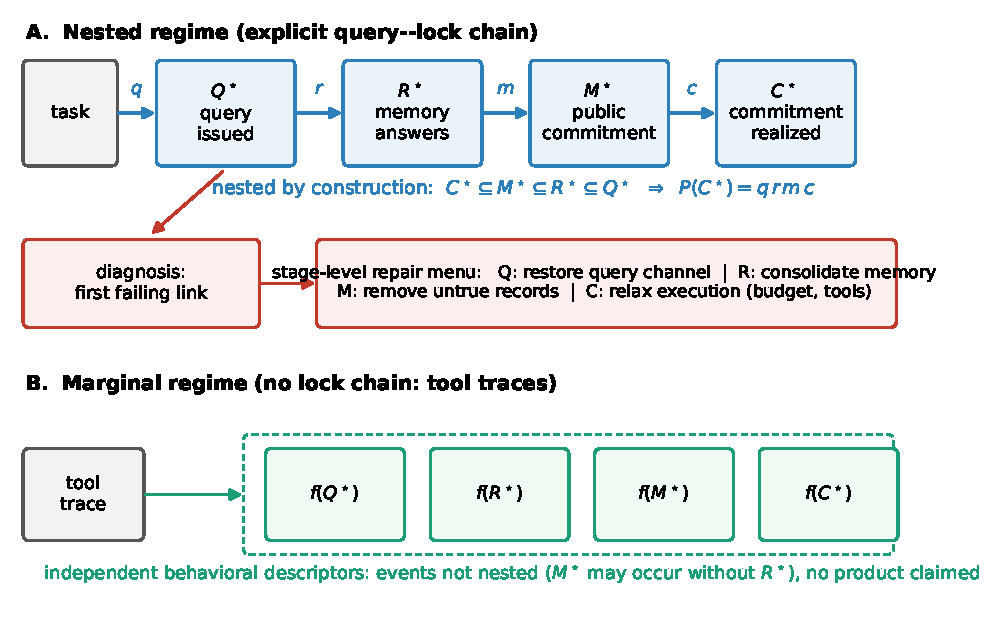
\includegraphics[width=.88\textwidth]{figures/fig_protocol_overview.pdf}
\caption{\qrmc{} evaluation contract. In the nested regime, the same attempt realizes Q, R, M, and C in order, yielding an exact chain-rule product for semantic-path completion. In the marginal regime, the same roles are reported as separate event frequencies. Stage diagnosis is used to select a targeted repair family.}
\label{fig:overview}
\end{figure}

\subsection{Constructs and observable events}

Figure~\ref{fig:overview} summarizes the contract, and Table~\ref{tab:constructs} states the constructs operationally. R and M require evaluator-side correspondence between memory records and task referents; without it, they cannot be interpreted as correctness events.

\begin{table}[t]
\caption{Constructs measured by \qrmc{}: logged event, required ground truth, and permitted inference.}
\label{tab:constructs}
\centering
\scriptsize
\setlength{\tabcolsep}{4pt}
\renewcommand{\arraystretch}{0.94}
\begin{tabular}{p{0.09\linewidth}p{0.24\linewidth}p{0.29\linewidth}p{0.27\linewidth}}
\toprule
Stage & Construct & Observable event and ground truth & Permitted inference \\
\midrule
Q & Query formation & A task-relevant query or intent is emitted. & The explicit memory channel was invoked with an evaluable request. \\
R & Retrieval satisfaction & The returned set contains a candidate satisfying the task predicate. & Task-relevant evidence was available through the queried memory interface. \\
M & Target materialization & The planner publicly commits to a true referent supported by the candidate set. & Retrieved evidence was converted into an actionable commitment. \\
C & Completion & The committed referent is reached or the committed tool action is realized. & Execution succeeded after the measured commitment. \\
\bottomrule
\end{tabular}
\end{table}

The definitions avoid latent deliberation claims. M is not ``the moment the agent decides,'' but the appearance of a public commitment in the trace; in a collective, that event can also change the environment by reserving or occupying a target.

\subsection{Nested and marginal measurement regimes}

When the runtime exposes an explicit query--retrieve--lock--execute chain, we define episode-level events so that a stage is counted only when one attempt realizes that stage together with its predecessors:
\begin{equation}
  \Cstar \subseteq \Mstar \subseteq \Rstar \subseteq \Qstar.
  \label{eq:nesting}
\end{equation}
Let
\begin{equation}
q=\Prob(\Qstar),\quad
r=\Prob(\Rstar\mid\Qstar),\quad
m=\Prob(\Mstar\mid\Rstar),\quad
c=\Prob(\Cstar\mid\Mstar).
\label{eq:rates}
\end{equation}
The nesting gives the exact identity
\begin{equation}
  \Prob(\Cstar)=qrmc.
  \label{eq:chain}
\end{equation}
No stage-Markov assumption is required for Equation~\ref{eq:chain}; it is the chain rule applied to nested events. The left-hand side is \emph{semantic-path completion}, not raw task success, which may also occur outside the explicit memory path.

The stronger interpretation is conditional. Treating $r$, $m$, or $c$ as a subsystem property requires relevant between-stage state to be represented in the logged context. Hidden query rewrites, memory updates, or side channels leave the identity intact but can distort the subsystem reading; our stress test finds the M--C contrast becomes unreliable first.

Tool-based agents that expose the roles but not a nested lock chain are reported through marginal frequencies $f(\Qstar),f(\Rstar),f(\Mstar),f(\Cstar)$. These marginals support fault localization but are never substituted into Equation~\ref{eq:chain}.

\subsection{From profile to diagnosis}

For the blinded study, the evaluator receives an anonymized stage profile and a labeled clean control from the same model--framework pair. A fixed first-failing-stage rule compares the profile with its control using thresholds selected before scoring. Structural failures directly remove a required interface event; behavioral failures perturb information or execution without mechanically forcing the target stage to zero. A second clean cell is held out to estimate false positives, and failed manipulation checks are excluded before scoring for every method.

The rule is deliberately simple: the purpose is to evaluate information carried by the stage representation, not to train a powerful classifier. We compare it with success-only, progress-milestone, two-stage retrieval/execution, first-deviation conformance, and learned logistic-regression diagnostics on the same anonymized aggregates.

\section{Validation Design}
\label{sec:design}

\subsection{Third-party agent stacks: blinded fault localization}

The primary study uses the same episodic household-memory task across an OpenAI SDK tool loop, LangGraph, and AutoGen. Each adapter records Q/R/M/C roles without modifying the model, and each cell contains 20 episodes. We repeat the study with \texttt{llama3.1:latest} and \texttt{qwen3:4b}. Ten fault types plus a held-out control produce 66 candidate model--framework cells; three \texttt{llama3.1:latest} prompt-only cells fail the manipulation check, leaving 63 scored cells. The decision rule, thresholds, exclusion condition, and repair mapping are fixed before labels are revealed.

The design separates structural faults, which test adapter semantics, from behavioral faults, which test localization when behavior remains stochastic and the affected event is not mechanically set to zero.

\subsection{Repair selection as decision validity}

A diagnosis is useful only if acting on it improves the system. We map each predicted stage to one repair family: restore the query channel (Q), restore or consolidate the relevant memory record (R), remove or disambiguate false target records (M), or relax execution with additional budget and reliable tools (C). For each fault--framework condition we run all four repair arms; the best arm is an oracle reference, not an input to the diagnostic.

Let $S_0$ be completion without repair, $S_d$ completion after the repair selected by diagnostic $d$, and $S_{\max}$ the best completion among the four available repair arms. We report mean gain $G_d=\mathbb{E}[S_d-S_0]$ and regret $R_d=\mathbb{E}[S_{\max}-S_d]$. The repair experiment contains 2,640 \texttt{llama3.1:latest} episodes; no-repair cells are reused from the blind study.

\subsection{Controlled intervention case studies}

The third-party benchmark is complemented by two settings in which stage interventions can be defined directly.

\paragraph{Single agent.}
Four semantic navigation task families are evaluated with 10 seeds and eight episodes per seed. Oracle-R, oracle-M, and oracle-C replace retrieval, target lock, and realization respectively, testing whether profiles distinguish upstream information from downstream execution bottlenecks.

\paragraph{Multi-agent collective.}
A scarce-target task is run under independent memory, shared memory, a central aggregator, and peer broadcast at $K\in\{1,2,4,8,16,32,48,64\}$ ticks. The 35,640-run sweep logs per-agent \qrmc{} events and separates own-evidence from peer-supported commitments. A reservation-and-rollback intervention keeps shared evidence while changing coordination, testing contention after commitment without removing information sharing.

\section{Results}
\label{sec:results}

\subsection{Blinded localization: event semantics are portable, behavioral diagnosis is imperfect}

\begin{figure}[t]
\centering
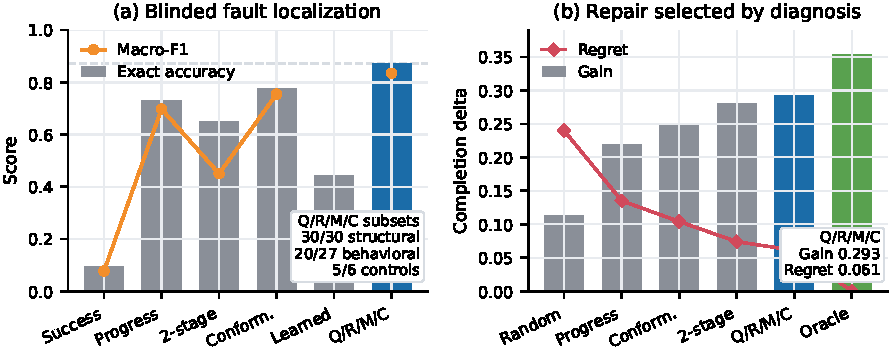
\includegraphics[width=.96\textwidth]{figures/fig_blind_repair_tae.pdf}
\caption{Primary TAE results. (a) Blinded fault localization compares evaluation resolutions on the same anonymized aggregates; the dashed line marks the two-stage side-level accuracy, while exact-stage scoring separates M from C. (b) Diagnoses are evaluated by the repair they select, with gain measured against the unrepaired condition and regret against the best available repair arm.}
\label{fig:blind-repair}
\end{figure}

Across the 63 scored cells, \qrmc{} makes 55 correct exact-stage decisions, for accuracy 0.873 and macro-F1 0.835 (Figure~\ref{fig:blind-repair}a). The five structural fault types are localized in all 30 model--framework cells; the held-out clean control is classified as ``none'' in five of six cells; and the behavioral subset is localized in 20/27 cells (0.741). This separation is the evidence against a purely circular interpretation in which the evaluator merely rediscovers an event that was directly disabled.

The structural checks behave as intended: removing the consolidated memory fact gives $f(\Rstar)=0$ in every affected cell, and tightening the tool budget gives $f(\Cstar)=0$ while Q and R remain present. Behavioral errors concentrate at Materialization. With \texttt{llama3.1:latest}, clean first-commitment accuracy is only 0.25--0.50, hiding additional M-stage perturbations under a control floor. With \texttt{qwen3:4b}, clean first-commitment accuracy rises to 0.90--0.95 on the OpenAI SDK tool loop and LangGraph, making the same perturbations detectable; AutoGen remains low at 0.40. Event semantics therefore transport more reliably than numerical stage profiles.

The two-stage retrieval/execution diagnostic reaches 0.873 if asked only to choose the correct side of the pipeline, but 0.651 at the original stage granularity, losing the M/C distinction. Conformance reaches 0.778 and misses budget-exhaustion cases where event order is preserved but conditional completion collapses. The learned classifier performs poorly on unseen fault types and labels every held-out control as faulty.

\subsection{Diagnoses are useful for repair, but fine-grained localization is not always necessary}

Figure~\ref{fig:blind-repair}b evaluates decision utility. \qrmc{} obtains mean completion gain 0.293 and regret 0.061, compared with the oracle-best gain 0.354. The improvement over the progress-milestone diagnostic is resolved by paired bootstrap ($\Delta G=+0.074$, 95\% CI $[+0.007,+0.157]$). The difference from the two-stage diagnostic is small and unresolved ($+0.013$, CI $[-0.009,+0.039]$). Thus the strongest supported statement is not that four stages always select a better repair. Four-stage resolution improves exact attribution and matches the strongest coarse diagnostic on downstream repair utility under the present repair menu.

The repair study also exposes the resolution limit of a stage label: restoring the true record under silent corruption recovers only 0.22--0.44 of the control gap because the corrupted record remains, while adding execution budget to a healthy OpenAI SDK tool-loop control lowers completion by 0.15.

\subsection{Sampling and threshold choices affect the evaluator itself}

We audit the evaluator by resampling the existing 20 episodes per scored cell, without new LLM trajectories. The deterministic reproduction script records input row-file hashes and computes from \texttt{rows\_meta\_llama.json} and \texttt{rows\_meta\_qwen.json}. Over 1000 without-replacement subsamples, mean exact-stage accuracy rises from 0.780 at $n=5$ to 0.829 at $n=10$, 0.852 at $n=15$, and 0.873 at $n=20$; diagnosis flip rate falls from 0.181 to 0.097, 0.050, and 0.000. Scaling R/M/C drop thresholds by 0.8, 0.9, 1.1, and 1.2 gives accuracies 0.889, 0.873, 0.825, and 0.825, so the conclusion is not a single-run accident but stricter thresholds reduce behavioral-fault recall.

\subsection{Controlled single-agent interventions separate upstream and downstream failures}

\begin{figure}[t]
\centering

\includegraphics[width=.90\textwidth]{figures/fig_oracle_waterfall.pdf}
\caption{Single-agent oracle interventions. Hazard recovery improves when retrieval is replaced by task-correct evidence, whereas goal-region rejoin exposes downstream failure after the semantic path is repaired.}
\label{fig:oracle}
\end{figure}

The navigation study checks interventions in a fully observable query--lock chain. In LavaGapS7 hazard recovery, oracle retrieval raises success from 0.39 to 0.60 (bootstrap 95\% CIs $[0.35,0.43]$ and $[0.51,0.69]$), with a positive per-seed delta for 9/10 seeds (sign test $p=0.004$). Oracle controller changes success much less, identifying an upstream retrieval/materialization bottleneck rather than a generic execution failure.

For goal-region rejoin, replacing retrieval restores semantic-path completion but leaves end-to-end success essentially unchanged. This is a downstream limitation: the retrieved semantic route can be repaired without solving the whole task. The distinction would be lost if $\Cstar$ were equated with raw task success.

Within-link inspection sharpens the retrieval diagnosis: when a candidate exists, ranking precision is 96.9\%, but the candidate set is empty at about 91\% of decision points under pooled, seed-weighted, and episode-weighted estimates. \qrmc{} localizes the stage; sub-stage cause requires finer logs.

\subsection{Multi-agent sharing moves the bottleneck, and a targeted coordination change moves it back}

\begin{figure}[t]
\centering
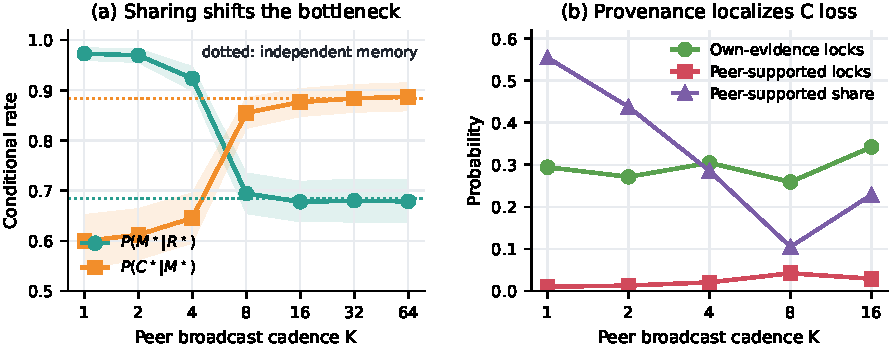
\includegraphics[width=.96\textwidth]{figures/fig_multiagent_tae.pdf}
\caption{Multi-agent mechanism case study. Faster peer broadcast increases materialization from retrieved evidence but lowers completion after materialization. Provenance localizes the completion loss to peer-supported locks, motivating the reservation-and-rollback intervention.}
\label{fig:multiagent}
\end{figure}

In the 35,640-run multi-agent sweep, retrieval is nearly saturated while Materialization and Completion move in opposite directions as peer broadcast becomes faster. Across 81 configuration cells, Spearman correlation between cadence $K$ and $\Prob(\Mstar\mid\Rstar)$ is $-0.53$ with cluster-robust CI $[-0.59,-0.47]$; for $\Prob(\Cstar\mid\Mstar)$ it is $+0.43$ with CI $[+0.37,+0.50]$. Faster sharing makes correct target materialization easier but a materialized target less likely to be completed.

Provenance shows the loss is concentrated in peer-supported locks. The reservation-and-rollback intervention keeps peer evidence while changing target coordination; under fast broadcast it raises unconditional success to 0.614--0.620, above the fixed $K=8$ peer baseline of 0.583. Across 18 matched cells the paired improvement is 0.037 with 95\% CI $[0.018,0.058]$, supporting contention after shared evidence is used.

The efficiency result is bounded: mean time-to-success among successful episodes has a shallow minimum at $K=8$ (7.63 ticks versus 8.04 for independent memory), but a censoring-aware summary gives a different ordering. The robust result is the direction of the two stage-specific changes, not a universal optimum.

\section{Validity Boundaries}
\label{sec:validity}

The reported rates are interpretable only under explicit measurement conditions. \textbf{Grounding:} R and M require evaluator-side correspondence between memory records and task referents. \textbf{Measurement regime:} Equation~\ref{eq:chain} applies only to nested query--lock traces; tool traces without that structure are marginals, not products. \textbf{Hidden state:} unlogged between-stage state can preserve the chain-rule identity while breaking causal attribution, so causal claims require richer logging or mechanism-targeted intervention. \textbf{Floors and thresholds:} an M-stage perturbation is hard to identify when clean M is already low, and stricter thresholds reduce recall for behavioral faults. \textbf{Resolution:} a low R or M rate identifies an interface, not an atomic cause; accumulation, ranking, grounding, ambiguity, and staleness require within-link instrumentation.

\section{Conclusion}

\qrmc{} evaluates explicit-memory agents through four observable commitments: query formation, retrieval satisfaction, materialization, and completion. The blinded benchmark shows portable stage semantics across three frameworks and two models; the repair experiment links diagnosis to downstream action; and the controlled interventions identify cases in which stage profiles track repairable mechanisms. The strongest reading is bounded: the nested product is an accounting identity, causal attribution requires additional assumptions or intervention, and exact localization need not dominate coarser diagnostics in repair utility. \qrmc{} is therefore an audit layer, not a substitute for task success.

\bibliographystyle{plainnat}
\bibliography{qrmc_tae_2026}

\appendix

\section{Operational Details}

\subsection{Episode-level events in the nested regime}
An episode may contain several query--retrieve--lock attempts. $\Qstar$ is one if an evaluable semantic intent is emitted. $\Rstar$ is one if at least one attempt contains a task-satisfying candidate together with its Q predecessor. $\Mstar$ is one if at least one such attempt produces a correct public commitment, and $\Cstar$ is one if that commitment is realized. This construction yields the nesting in Equation~\ref{eq:nesting}. It is intentionally stricter than recording whether an event of the same type appeared somewhere in the episode without a shared attempt lineage.

\subsection{Fault-benchmark accounting}
The blind set contains ten fault types plus an additional clean control, crossed with three frameworks and two models. The nominal design therefore has 66 cells. A prompt-only fault fails its pre-specified manipulation check in three \texttt{llama3.1:latest} framework cells; those cells are removed for every method before labels are scored, yielding 63 cells. Of the retained cells, 30 correspond to five structural fault types, six are held-out controls, and 27 are behavioral faults. \qrmc{} classifies 55/63 cells correctly: 30/30 structural, 5/6 controls, and 20/27 behavioral.

\subsection{Diagnostic comparison}
The success-only reference labels a cell as fault-free only when completion remains within its control range; it cannot distinguish stages. The progress-milestone rule reads the stage frequencies as an ordered progress vector. The two-stage rule collapses Q/R into an information side and M/C into an action side. The conformance rule reports the first deviation from the canonical event sequence. The learned baseline is logistic regression trained on labeled fault examples and evaluated on fault types excluded from its training set. All rule-based thresholds are fixed before the blind labels are scored.

\section{Additional Controlled Results}

\subsection{Single-agent oracle pattern}
Hazard recovery is the clearest upstream intervention result. Base success is 0.39; oracle-R reaches 0.60, oracle-M produces a comparable improvement, and oracle-C changes success only modestly. Goal-region rejoin shows the complementary pattern: repairing the semantic retrieval path does not repair raw task success. The distinction motivates reporting $\Cstar$ separately from the task-level outcome.

\subsection{Multi-agent mechanism check}
The peer-broadcast study changes two quantities together as cadence increases: the freshness of peer evidence and the probability that multiple agents pursue the same scarce target. Provenance stratification identifies the completion loss among peer-supported locks. The reservation-and-rollback intervention preserves fast evidence exchange but prevents an occupied target from remaining an uncoordinated shared commitment. The resulting improvement is therefore a mechanism-targeted check of the M--C interpretation, not simply another communication architecture comparison.

\section{Reproducibility and Reporting Notes}
All headline fault-localization decisions use 20 episodes per cell. Fault labels are hidden from the diagnostic rule until after predictions are written. One labeled clean control is used for calibration; a second clean control is included in the blind set. Cells that fail a pre-specified manipulation check are excluded for all methods rather than re-labeled after observing diagnostic performance. The external fault benchmark uses Ollama model identifiers \texttt{llama3.1:latest} and \texttt{qwen3:4b}, with local Ollama model IDs \texttt{46e0c10c039e} and \texttt{359d7dd4bcda}, respectively. The OpenAI condition is a Python OpenAI SDK Chat Completions tool loop pointed at Ollama's OpenAI-compatible endpoint. Multi-agent effect intervals are cluster-robust over design cells; single-agent oracle comparisons use seed-level pairing where reported in the main text. The numerical results in this submission are inherited from fixed experimental records and deterministic analysis scripts.

\end{document}
